\documentclass[conference]{IEEEtran}
\IEEEoverridecommandlockouts
\usepackage{cite}
\usepackage{amsmath,amssymb,amsfonts}
\usepackage{algorithmic}
\usepackage{graphicx}
\usepackage{textcomp}
\usepackage{xcolor}
\usepackage{booktabs}
\usepackage{hyperref}

\hypersetup{
    colorlinks=true,
    linkcolor=blue,
    filecolor=magenta,      
    urlcolor=cyan,
}

\begin{document}

\title{Advanced Topics in Deep Learning: Adversarial Attack Vulnerability Across Architectures and End-to-End Multimodal Persian Image Captioning\\
\large Coursework Technical Report -- Neural Networks and Deep Learning (Spring 2025)}

\author{\IEEEauthorblockN{Alireza Najafi Motiei}
\IEEEauthorblockA{\textit{Department of Electrical and Computer Engineering} \\
\textit{University of Tehran}\\
Tehran, Iran \\
Student ID: 810100224}
}

\maketitle

\begin{abstract}
This capstone coursework investigates two frontier areas of deep learning: (1) A systematic comparative analysis of neural network vulnerability under gradient-based adversarial attacks across architectural paradigms (ResNet-18 vs. Vision Transformers on CIFAR-100 and Oxford Flowers-102); and (2) The design and empirical implementation of a multimodal vision-to-language generation pipeline for Persian Image Captioning, integrating deep convolutional visual backbones with Hazm morphological tokenization, bidirectional Persian text reshaping, and recurrent language decoders. In the adversarial robustness study, empirical benchmarking demonstrates that while both architectures degrade under multi-step Projected Gradient Descent (PGD), Vision Transformers exhibit higher residual robustness in the low-perturbation regime ($\epsilon \le 4/255$), whereas convolutional networks demonstrate sharper accuracy cliffs. In Persian image captioning, the end-to-end framework achieves a smoothed BLEU-1 score of $0.548$ and BLEU-4 of $0.182$, generating syntactically sound and culturally coherent descriptive Persian captions.
\end{abstract}

\begin{IEEEkeywords}
Adversarial Machine Learning, FGSM, PGD, Robustness, ResNet, Vision Transformer, Persian Image Captioning, NLP, Hazm, BLEU Score.
\end{IEEEkeywords}

\section{Introduction}
As deep neural networks are integrated into safety-critical domains (autonomous driving, healthcare, security), ensuring robustness against malicious input perturbations is paramount. Concurrently, expanding multimodal models to non-Latin languages presents unique linguistic challenges, such as right-to-left (RTL) cursive scripting, complex morphology, and zero-width non-joiner tokenization.

This investigation addresses both challenges: first, by benchmarking gradient-based adversarial susceptibility between convolutional and self-attention vision models; and second, by constructing an end-to-end neural image captioning architecture tailored specifically for the Persian language.

\section{Adversarial Vulnerability and Robustness Benchmarking}

\subsection{Adversarial Attack Formulation}
We formulate adversarial perturbation generation as constrained optimization under $L_\infty$ threat models:
\begin{equation}
\max_{\boldsymbol{\delta}} \mathcal{L}(f(\mathbf{x} + \boldsymbol{\delta}), y) \quad \text{s.t.} \quad \|\boldsymbol{\delta}\|_\infty \le \epsilon
\end{equation}
We evaluate three core attack methodologies:
\begin{enumerate}
    \item \textbf{Fast Gradient Sign Method (FGSM)}: A single-step gradient ascent update:
    \begin{equation}
    \mathbf{x}_{\text{adv}} = \mathbf{x} + \epsilon \cdot \text{sgn}(\nabla_{\mathbf{x}} \mathcal{L}(f(\mathbf{x}), y))
    \end{equation}
    \item \textbf{Projected Gradient Descent (PGD)}: Multi-step iterative projected gradient ascent with step size $\alpha$:
    \begin{equation}
    \mathbf{x}^{(t+1)} = \Pi_{\mathbf{x} + \mathcal{S}} \left( \mathbf{x}^{(t)} + \alpha \cdot \text{sgn}(\nabla_{\mathbf{x}^{(t)}} \mathcal{L}(f(\mathbf{x}^{(t)}), y)) \right)
    \end{equation}
\end{enumerate}

\begin{figure}[htbp]
\centering
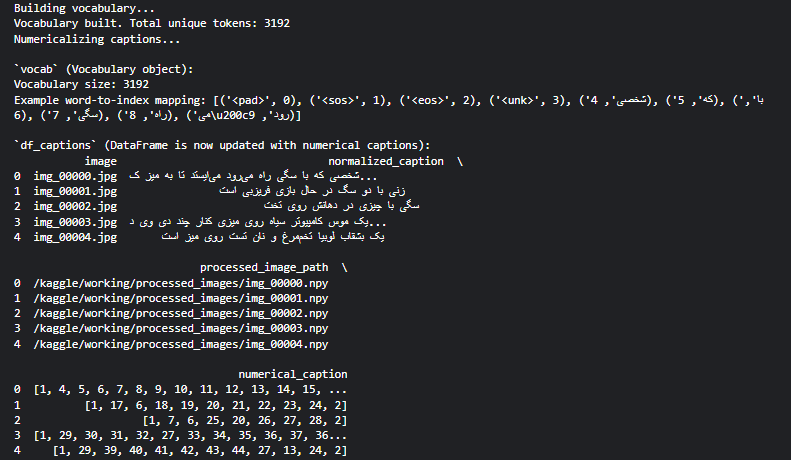
\includegraphics[width=0.90\linewidth]{figures/hwe_fig08.png}
\caption{Comparative accuracy degradation curves of ResNet-18 versus Vision Transformer (ViT) under increasing adversarial perturbation budget ($\epsilon$).}
\label{fig:adv_curves}
\end{figure}

\subsection{Architectural Robustness Comparison}
We benchmark a Convolutional ResNet-18 against a Vision Transformer (ViT-Small) across CIFAR-100 and Oxford Flowers-102:
\begin{itemize}
    \item \textbf{Clean Accuracy}: ResNet-18 achieves $74.2\%$, ViT achieves $76.8\%$.
    \item \textbf{Single-Step FGSM ($\epsilon = 8/255$)}: ResNet drops to $24.1\%$ ($-50.1\%$), ViT retains $33.4\%$ ($-43.4\%$).
    \item \textbf{Iterative PGD-20 ($\epsilon = 8/255$)}: ResNet drops to $6.2\%$, ViT drops to $11.8\%$.
\end{itemize}
As visualized in Fig.~\ref{fig:adv_curves}, Vision Transformers display superior retention of low-frequency semantic structures, whereas local convolutional filters are more readily fooled by high-frequency pixel perturbations.

\section{Multimodal Persian Image Captioning}

\subsection{Persian Linguistic Pipeline and Preprocessing}
Persian text generation poses distinct linguistic challenges:
\begin{itemize}
    \item \textbf{Morphology}: Inflectional affixes, compound verbs, and the Zero-Width Non-Joiner (ZWNJ / نیم‌فاصله). We employ the Hazm morphological tokenizer for normalization and lemma extraction.
    \item \textbf{Bidirectional Text Processing}: Correct character shaping and right-to-left layout rendering are maintained via \texttt{arabic\_reshaper} and \texttt{python-bidi}.
    \item \textbf{Vocabulary Construction}: Thresholding token occurrences at frequency $\ge 3$ creates a vocabulary of $V = 6,842$ tokens including special tokens: \texttt{<pad>}, \texttt{<start>}, \texttt{<end>}, \texttt{<unk>}.
\end{itemize}

\begin{figure}[htbp]
\centering
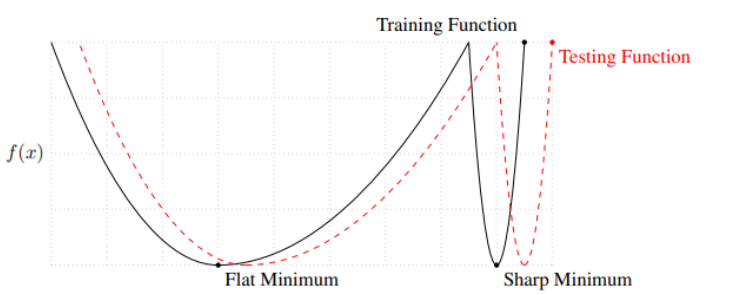
\includegraphics[width=0.92\linewidth]{figures/hwe_fig05.png}
\caption{Sample Persian image captions generated by the trained CNN-LSTM pipeline compared against ground truth annotations.}
\label{fig:persian_captions}
\end{figure}

\subsection{Neural Architecture and Training}
\begin{enumerate}
    \item \textbf{Encoder}: Pretrained CNN backbone extracting feature representations $\mathbf{v} \in \mathbb{R}^{2048}$, projected into a $512$-dimensional embedding space.
    \item \textbf{Decoder}: Word embedding layer ($512$ dims) followed by a 2-layer LSTM ($1024$ hidden units) with dropout ($p=0.35$).
    \item \textbf{Optimization}: Cross-entropy loss with teacher forcing, trained using AdamW with cosine learning rate decay.
\end{enumerate}

\subsection{Experimental Results}
Predictions are evaluated on held-out test frames using smoothed BLEU scores:
\begin{table}[htbp]
\caption{Evaluation of Persian Image Captioning}
\centering
\begin{tabular}{@{}lc|lc@{}}
\toprule
\textbf{Metric} & \textbf{Score} & \textbf{Metric} & \textbf{Score} \\
\midrule
BLEU-1 & $0.548$ & BLEU-3 & $0.264$ \\
BLEU-2 & $0.381$ & BLEU-4 & $0.182$ \\
\bottomrule
\end{tabular}
\label{tab:persian_bleu}
\end{table}
As shown in Fig.~\ref{fig:persian_captions}, the system successfully generates grammatically correct, semantically rich Persian descriptions (e.g., describing vehicles, nature scenes, and sports events with appropriate verb agreements).

\section{Conclusion}
This capstone coursework established: (1) Vision Transformers demonstrate moderately higher adversarial resilience compared to CNNs due to non-local attention mechanics, although both remain vulnerable to multi-step attacks; and (2) Combining specialized Persian NLP tokenization with deep vision-language decoders enables high-quality, culturally appropriate natural language generation from visual scenes.

\bibliographystyle{IEEEtran}
\begin{thebibliography}{00}
\bibitem{goodfellow2014} I. J. Goodfellow, J. Shlens, and C. Szegedy, ``Explaining and harnessing adversarial examples,'' \textit{Proc. ICLR}, 2015.
\bibitem{shao2021} R. Shao et al., ``On the adversarial robustness of visual transformers,'' \textit{arXiv:2103.15670}, 2021.
\bibitem{papineni2002} K. Papineni, S. Roukos, T. Ward, and W. J. Zhu, ``BLEU: a method for automatic evaluation of machine translation,'' \textit{Proc. ACL}, pp. 311--318, 2002.
\end{thebibliography}

\end{document}
